\documentclass[border=10pt]{standalone}

\usepackage{tikz}
\usepackage{tikzsymbols}
\usetikzlibrary{calc,patterns,shapes.geometric}

\def\centerarc[#1](#2)(#3:#4:#5){\draw[#1] ($(#2)+({#5*cos(#3)},{#5*sin(#3)})$) arc (#3:#4:#5);}

\begin{document}
	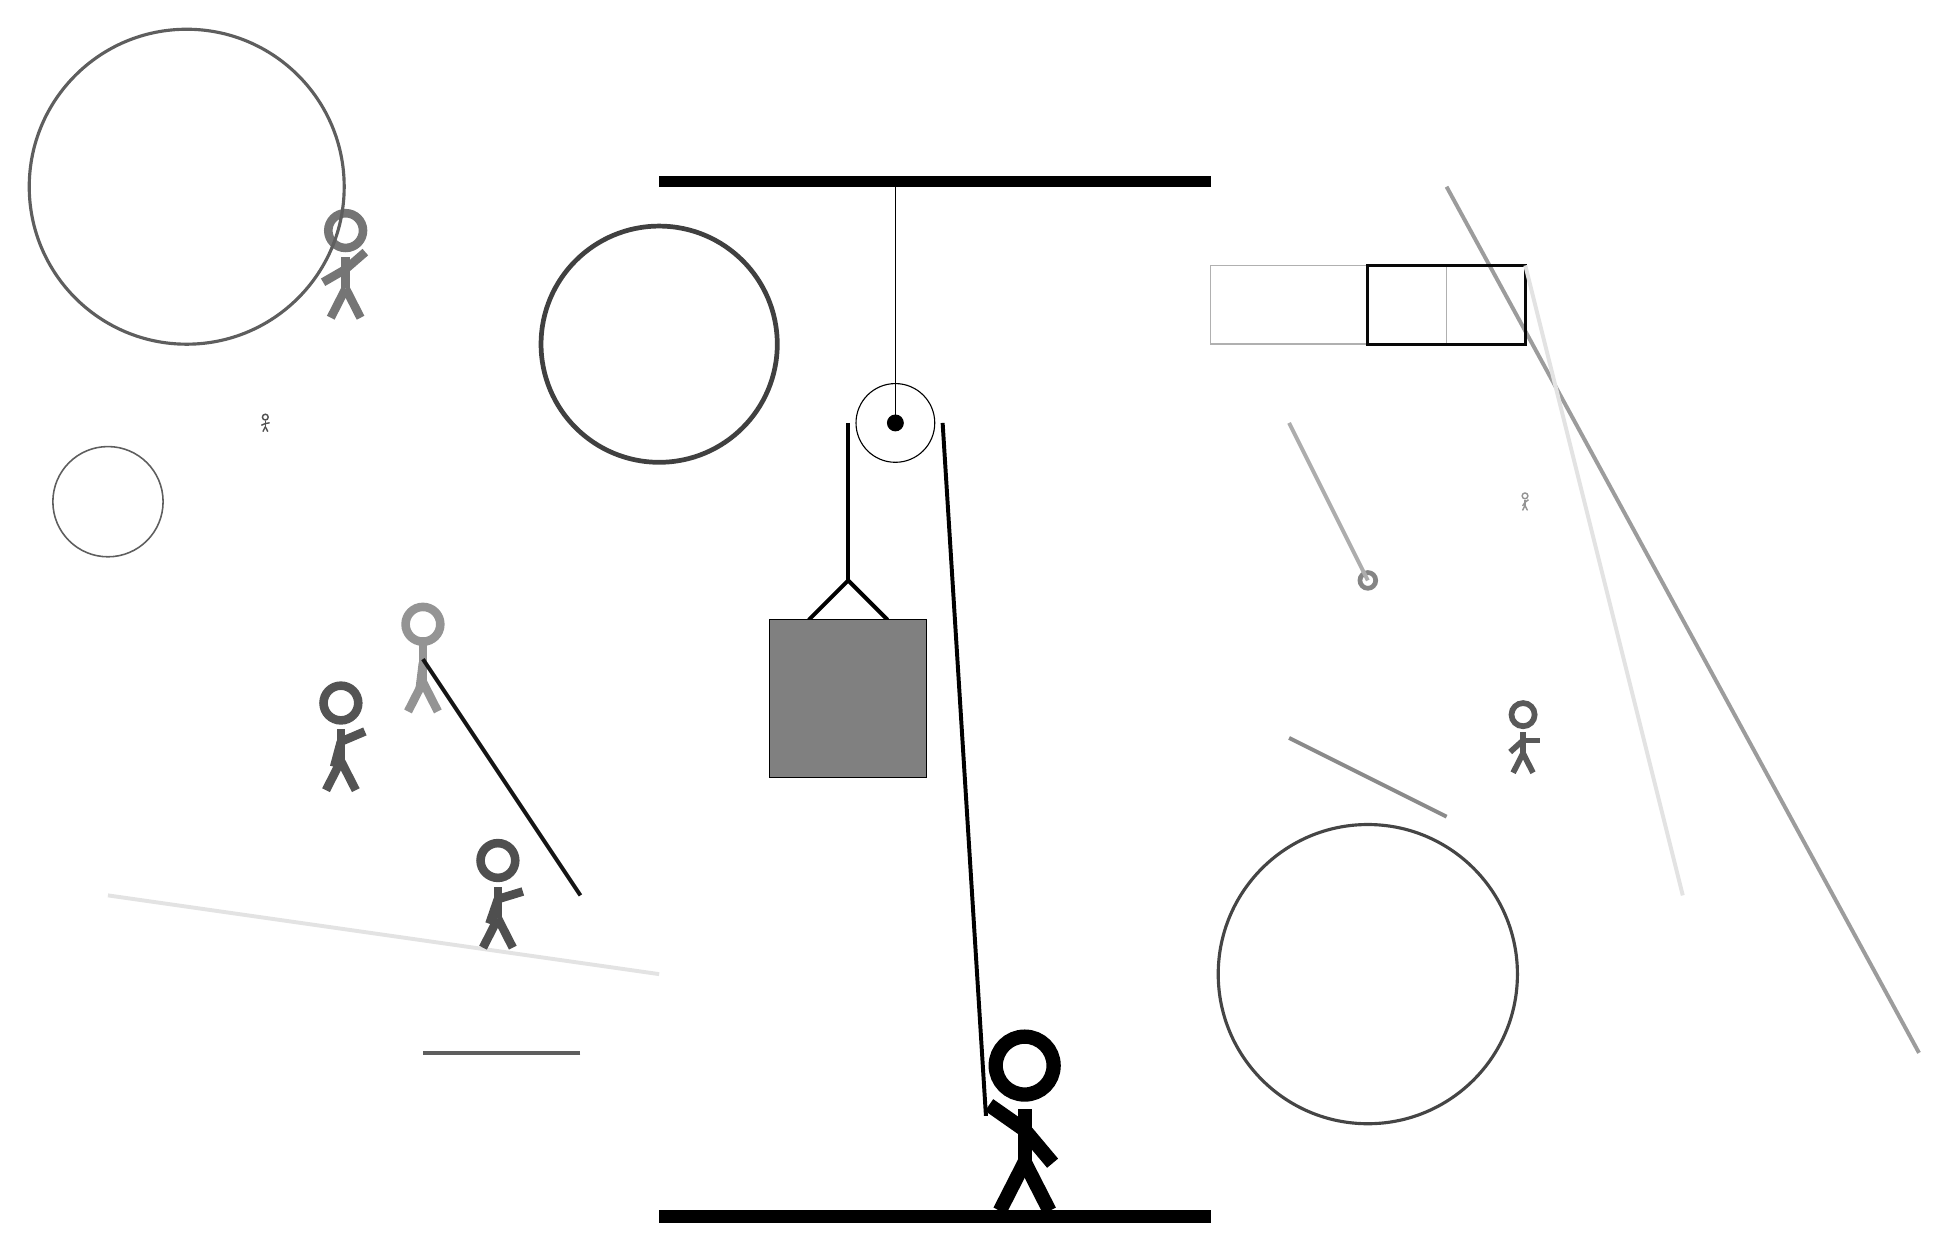
\begin{tikzpicture}
		%%%%% START %%%%%
		
		\draw[fill=black] (-2, 10) rectangle (5, 10.125);
		
		\draw (1, 7) circle (0.5);
		\draw[fill=black] (1, 7) circle (0.1);
		\draw (1, 10) -- (1, 7);
		
		\draw[line width=0.5mm] (-0.1, 4.5) -- (0.4, 5.0) -- (0.9, 4.5);
		\draw[fill=black!50] (-0.6, 4.5) rectangle (1.4, 2.5);
		
		\draw[line width=0.5mm] (0.4, 7) -- (0.4, 5.0);
		\centerarc[line width=0.5mm](1, 7)(0:180:0.6);
		\draw[line width=0.5mm](1.6, 7) -- (2.15, -1.8);
		
		\node[line width=0.2mm, color=black!42] at (-5, 4) {\Strichmaxerl[6][83][90]};
		
		\draw[line width=0.5mm, color=black!92](-5, 4) -- (-3, 1);
		\draw[line width=0.5mm, color=black!39](8, 10) -- (14, -1);
		\draw[line width=0.2mm, color=black!31] (5, 8) rectangle (8, 9);
		\node[line width=0.5mm, color=black!54] at (-6, 9) {\Strichmaxerl[6][30][41]};
		
		\node[line width=0.3mm, color=black!65] at (9, 3) {\Strichmaxerl[4][42][0]};
		
		\draw[line width=0.5mm, color=black!11](-2, 0) -- (-9, 1);
		\draw [line width=0.4mm, color=black!73](7, 0) circle (1.9);
		\draw [line width=0.6mm, color=black!48](7, 5) circle (0.1);
		\draw [line width=0.4mm, color=black!63](-8, 10) circle (2.0);
		
		\draw[line width=0.4mm, color=black!97] (7, 8) rectangle (9, 9);
		\draw [line width=0.2mm, color=black!63](-9, 6) circle (0.7);
		\draw[line width=0.5mm, color=black!11](9, 9) -- (11, 1);
		
		\draw[line width=0.5mm, color=black!63](-3, -1) -- (-5, -1);
		\draw [line width=0.6mm, color=black!75](-2, 8) circle (1.5);
		\node[line width=0.4mm, color=black!69] at (-4, 1) {\Strichmaxerl[6][71][17]};
		
		\node[line width=0.5mm, color=black!67] at (-6, 3) {\Strichmaxerl[6][75][23]};
		
		\node[line width=0.2mm, color=black!42] at (9, 6) {\Strichmaxerl[1][56][37]};
		\node[line width=0.4mm, color=black!68] at (-7, 7) {\Strichmaxerl[1][23][10]};
		\draw[line width=0.5mm, color=black!32](6, 7) -- (7, 5);
		\draw[line width=0.5mm, color=black!46](6, 3) -- (8, 2);
		
		\node at (2.6, -1.9) {\Strichmaxerl[10][-35][-50]};
		
		\draw[fill=black] (-2, -3) rectangle (5, -3.15);
		
		%%%%% END %%%%%
	\end{tikzpicture}
\end{document}